\section{Experiments}

We will in this section present the results of our performance experiments and demonstrate that our method performs well both when considering the Proxy and Server scenario [REF TO PREV. SEC. NEEDED]. 

We have implemented SPC, our method, with the 3 cache representation schemes - List cache, Graph cache, Compressed Graph cache - described in section [REF NEEDED].

To compare how well we have done, we have implemented two baseline competitors, LRU and HQF. LRU is a dynamic caching method which evicts the Least recently used cache item if there is no space in the cache for new entries. HQF adds to the cache, the \spaths from the most frequent start-/end-points in the training data. This is the most common usage of static caching in the web caching literature [CITE NEEDED].






% In this section, we present the results of performance
% experiments, demonstrating the efficiency and realworld applicability of the proposed algorithms. We
% have implemented a prototype of VICINITYLOCATOR,
% as well as Hide&Crypt [5], and FRIENDLOCATOR
% [7] for comparison. For simplicity in comparing the
% three implementations,  contains granularities as grids
% with uniform squares, where edge length B(l) depends
% on level l. We set B(l) = L0  2
% l
% where L0 is the cell
% width at level 0. L(l) = B(l)
% p
% 2 in this case
\subsection{Query Sources \& Generation}

To be filled out when we have actually done some more tests on synthetic data. 

How do we generate queries and why do we generate as we do.

Which historical query datasets do we have, and what is their size and origin.

- Aalborg: Query workload from and around the Danish city of Aalborg

- Beijing: Query workload from Beijing

- Oldenburg: Synthetic data generated on the German city of Oldenburg, using the Brinkhoff datagenerator \cite{brinkhoff} 



\subsection{Experimental Setting}

% - Which parameters are common for all tests
% - What are the ranges/values each parameter can take.
% - Which parameters are set to a default value unless otherwise stated (and what are the default values)
% - Which methods, and in which configuration, do we consider.
% 
% SPC: level/partitions
% ALL: cacehe size
% HQF, SPC: cache type
% ALL: Map/dataset
% ALL: number of queries

Our 3 caching methods, SPC, HQF, and LRU, share a number of common settings which, unless stated otherwise, will be set to their default values: 
The number of levels in the kD-tree are (i.e. 16.384 regions). We will use the list cache representation as the default cache representation, where each vertex use one byte. The default cache size is set to 160.000 bytes.

Except for tests on synthetic data, the size of training and test query datasets are given already. The size of each dataset, as well as the map they are captured on, is given in table \ref{tab:datasetsize}.

We do not give a default size for the query-datasets/ Maps, as we will execute all of our tests, described in section \ref{subsec:expProxy} and \ref{subsec:expServer}, for each dataset.


\begin{table}
\center
\begin{tabular}{|l|l|l|}\hline
Dataset & $\#$Training Queries & $\#$Vertices in Map \\\hline
Aalborg & 1643 & 136347 \\\hline
Beijing & 6478 & 79603 \\\hline
\end{tabular}
\caption{Size of query datasets. Training and testing datasets are of equal size.}
\label{tab:datasetsize}
\end{table}


\subsection{Proxy}\label{subsec:expProxy}

On the proxy [REF FIGURE/SECTION] we won't be doing \spath calculations, so the most important performance measure is the cache hit ratio.

For both the Aalborg and Beijing dataset we vary the cache size and number of levels to show the impact on the cache hit ratio. We have implemented a number of optimizations to the cache storage [REF PREV SEC. NEEDED] and we will show their impact on the cache hit ratio.



\subsubsection{Cache Size}




\begin{figure}[htb]
\center
  \begin{tabular}{cc}
     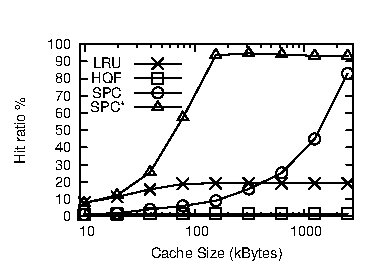
\includegraphics[width=0.5\columnwidth]{figures/aalborgHitVsCacheSize.pdf}
     &
     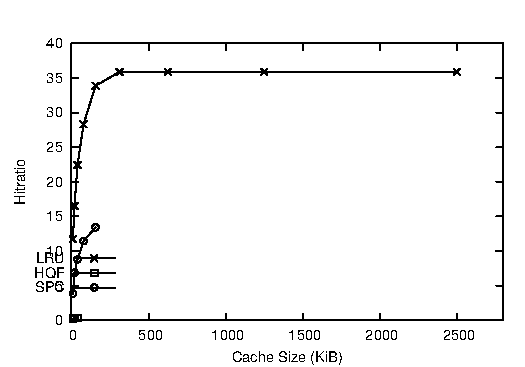
\includegraphics[width=0.5\columnwidth]{figures/beijingHitVsCacheSize.pdf}
      \\
     (a) Aalborg data & (b)  Beijing data
     \end{tabular} 
\caption{Hit ratio vs. cache size }
\label{fig:cSizeVsHitRatio}
\end{figure}

\begin{itemize}
\item We can see $SPC^*$ performs much better than competitors
\item  LRU perform well on small cache sizes, but the cache hit ratio quickly level out and stop growing, thus LRU is not scalable.
\item 
\end{itemize}


\subsubsection{SPC Levels}



\begin{figure}[htb]
\center
  \begin{tabular}{ccc}
     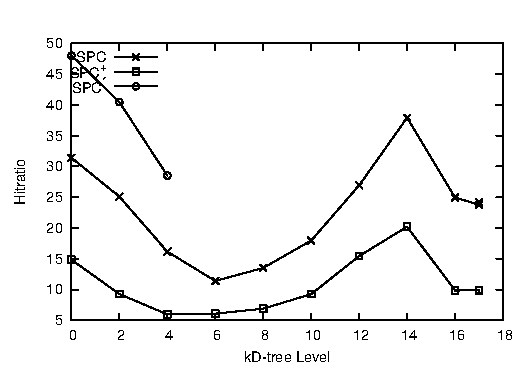
\includegraphics[width=0.5\columnwidth]{figures/aalborgHitVsLevel.pdf}
     &
     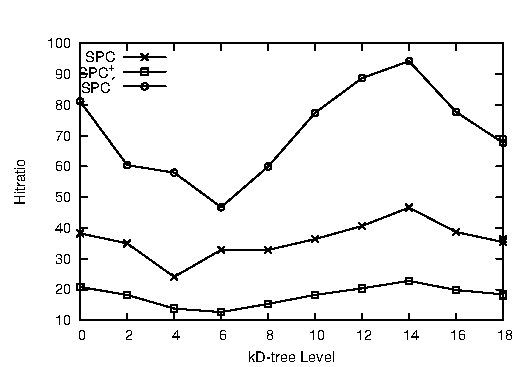
\includegraphics[width=0.5\columnwidth]{figures/beijingHitVsLevel.pdf}
      \\
     (a) Aalborg data & (b)  Beijing data
     \end{tabular}
\caption{Hit ratio vs. Levels}
\label{fig:levelVsHitRatio}
\end{figure}



\subsubsection{Vary Training data size}





\begin{figure}[htb]
\center
     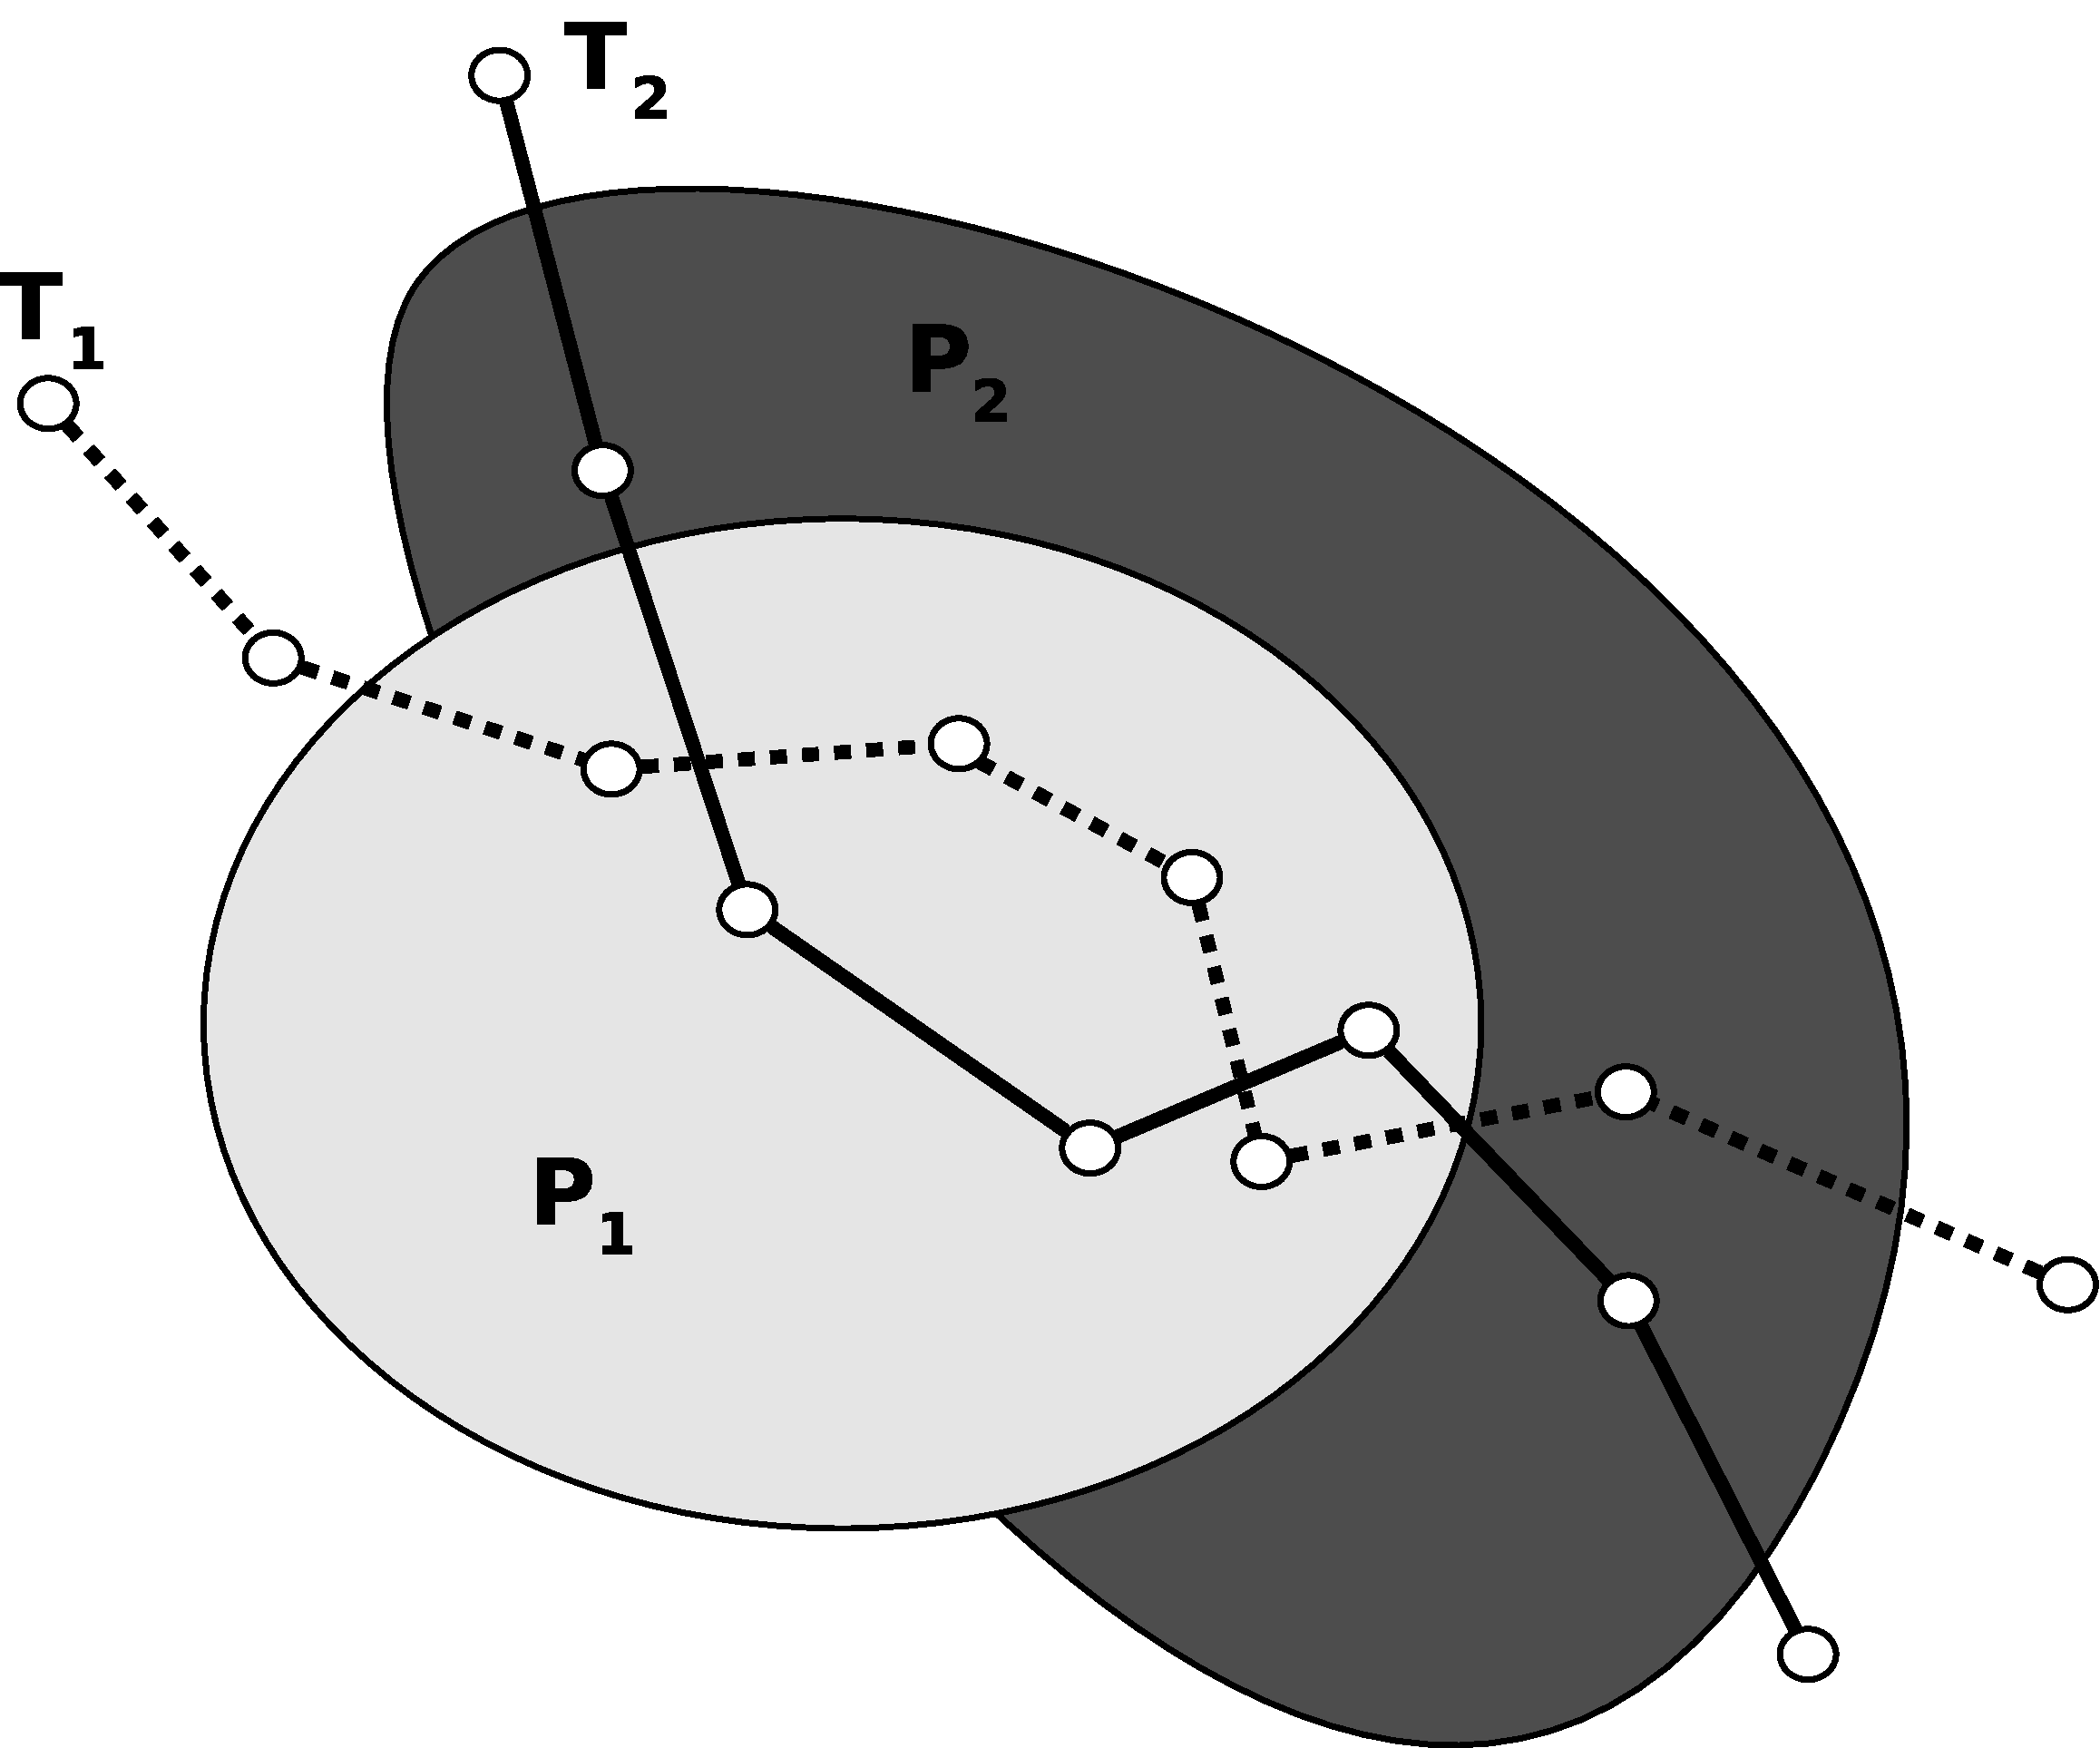
\includegraphics[width=0.5\columnwidth]{figures/poiIntersect.pdf}
\caption{ Hit ratio vs. training data size}
\label{fig:dataSizeVsHitRatio}
\end{figure}
% \noindent
% \begin{tabular}{|l |p{0.58\columnwidth} |l |}
% \hline
% \textbf{Parameter} & \textbf{Meaning / used for} & \textbf{Standard value} \\\hline
% Mapfile & The map which the test is performed on & \\\hline
% NumQueries & Number of \spath queries in test & \\\hline
% QuerySet & which dataset is used to provide queries & \\\hline
% TrainSet & For generating region statistics, which dataset is used & \\\hline
% CacheSize & Size of cache in bits & \\\hline
% cacheType & Type of cache representation (list/graph) & \\\hline
% kD-tree & Hight of the kD-tree & \\\hline
% avgLenght & Average length of a shortest path & \\\hline
% \end{tabular}

% Write experiments to examine performance of goal 1 \& 2 
% Test ideas (several ideas may be combined, like item 1 can be done on all datasets from item 2):\\
% \begin{itemize}
% \item increase kd-tree hight from 0-18
% \item different maps [Oldenburg, Aalborg, Beijing]
% \item compare cache type performance
% \item compare with baseline methods. [LRU dynamic, Dynamic(maxLevel)]
% \item vary the cache size [10.000-2560000]
% \item vary number of queries. [only for synthetic data]
% \end{itemize}
\subsection{Server}\label{subsec:expServer}

On the server [REF TO FIGURE] our aim is slightly different than on the Proxy, as we also have to consider that there may be some paths that are so small that it may be cheaper to simply re-calculate the result, in stead of caching it.

For the Server scenario we will estimate 
$\Gamma(P_{a,b})$ 
[REF TO EQUATION], the benefit of a path, as 
$\Gamma_E(P_{a,b})$:


\begin{equation} \label{eq:estimateCost}
\Gamma{_E} (P_{a,b})  =\sum\limits_{P_{a,b} \in \mathfrak{U}(P_{a,b})} |SP_{a,b}|^2
\end{equation}

% On the proxy server we won't be doing \spath calculations, so the most important performance measure is the cache hit ratio.
% 
% For both the Aalborg and Beijing dataset we vary the cache size and number of levels to show the impact on the cache hit ratio. We have implemented a number of optimizations to the cache storage [REF PREV SEC. NEEDED] and we will show their impact on the cache hit ratio.



\begin{tabular}{|l|r|r|r|}\hline
AA-Method & Time & Hit ratio & Vertices visited \\\hline
SPC-P & 28.87 & 99 & 23981137 \\\hline
SPC$^+$-P & 23.74 & 375 & 20570981 \\\hline
SPC$^*$-P & 22.11 & 1539 & 5559029\\\hline
SPC-S & 31.87 & 60 & 24023852 \\\hline
SPC$^+$-S & 7.16 & 1549 & 5201386 \\\hline 
SPC$^*$-S & 22.11 & 1539 & 5559029 \\\hline
\end{tabular}



\begin{tabular}{|l|r|r|r|}\hline
BJ-Method & Time & Hit ratio & Vertices visited \\\hline
SPC-P & 94.58 & 5738 & 85810602\\\hline
SPC$^+$-P & 89.44 & 1310 & 82122187 \\\hline
SPC$^*$-P & &  &  \\\hline
SPC-S & 93.22 & 97 & 86753995 \\\hline
SPC$^+$-S & 84.74 & 717 & 79557276 \\\hline 
SPC$^*$-S &  &  &  \\\hline
\end{tabular}





\begin{figure}[htb]
\center
  \begin{tabular}{cc}
     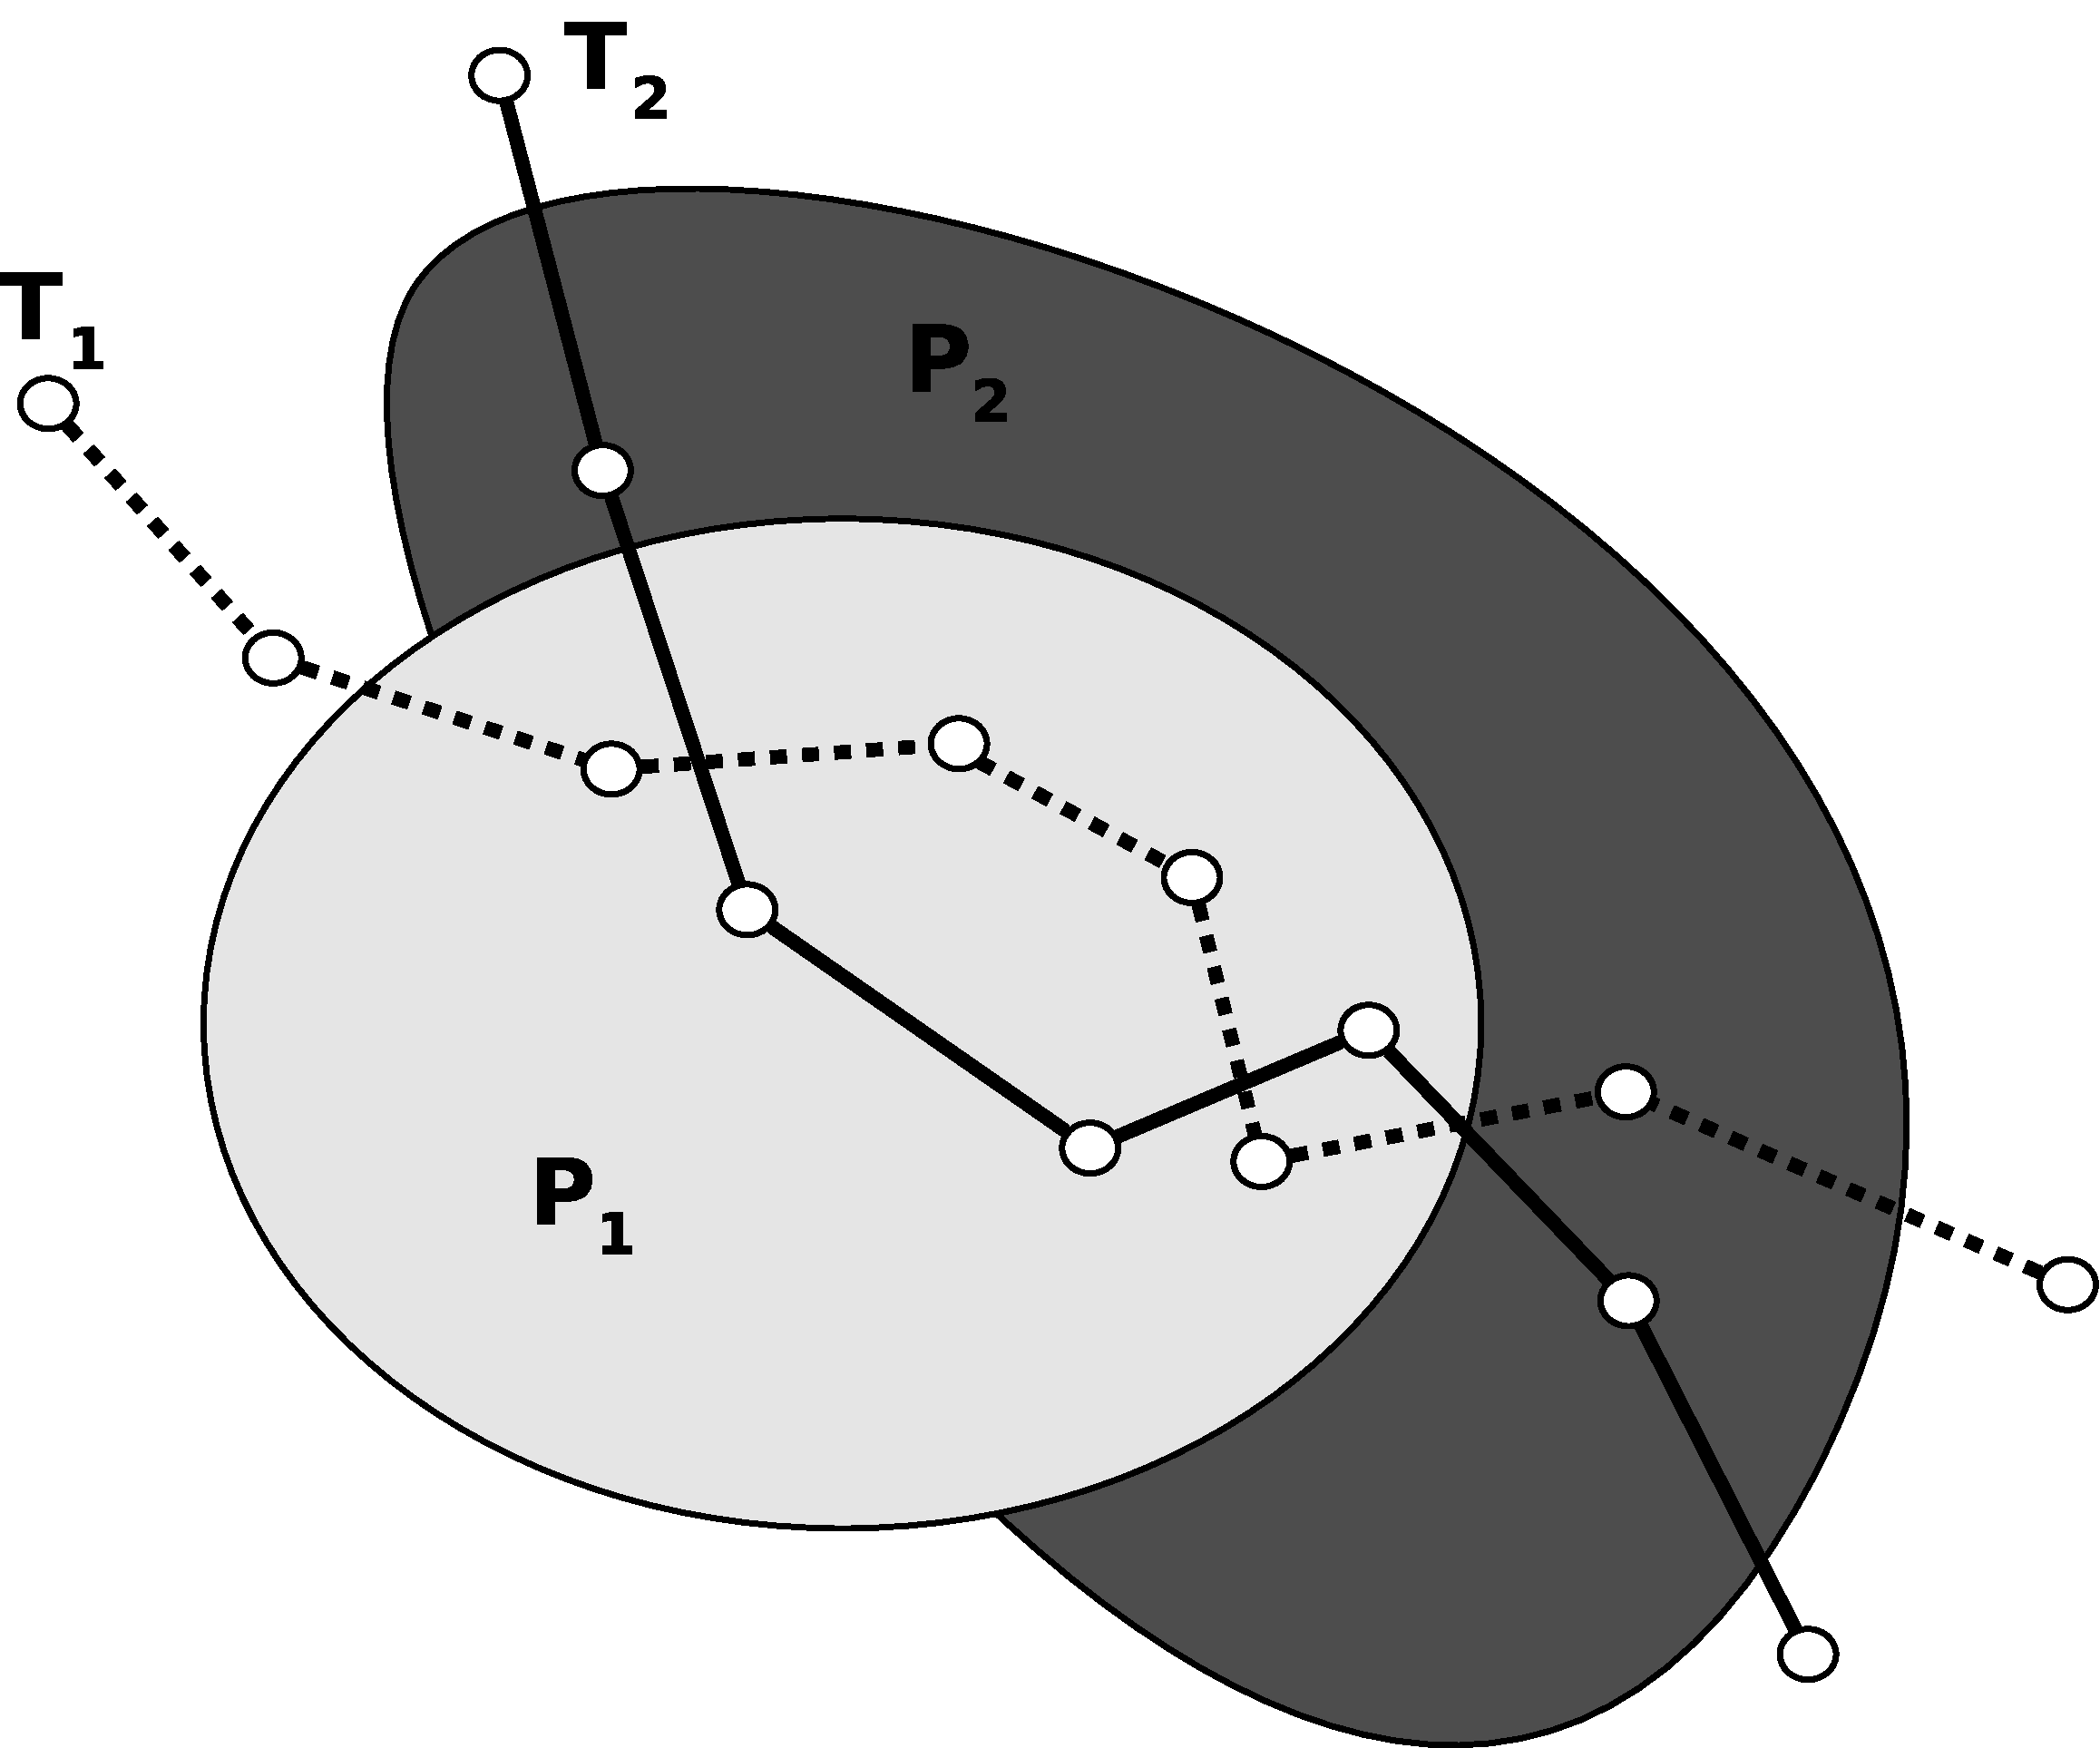
\includegraphics[width=0.3\columnwidth]{figures/poiIntersect.pdf}
     &
     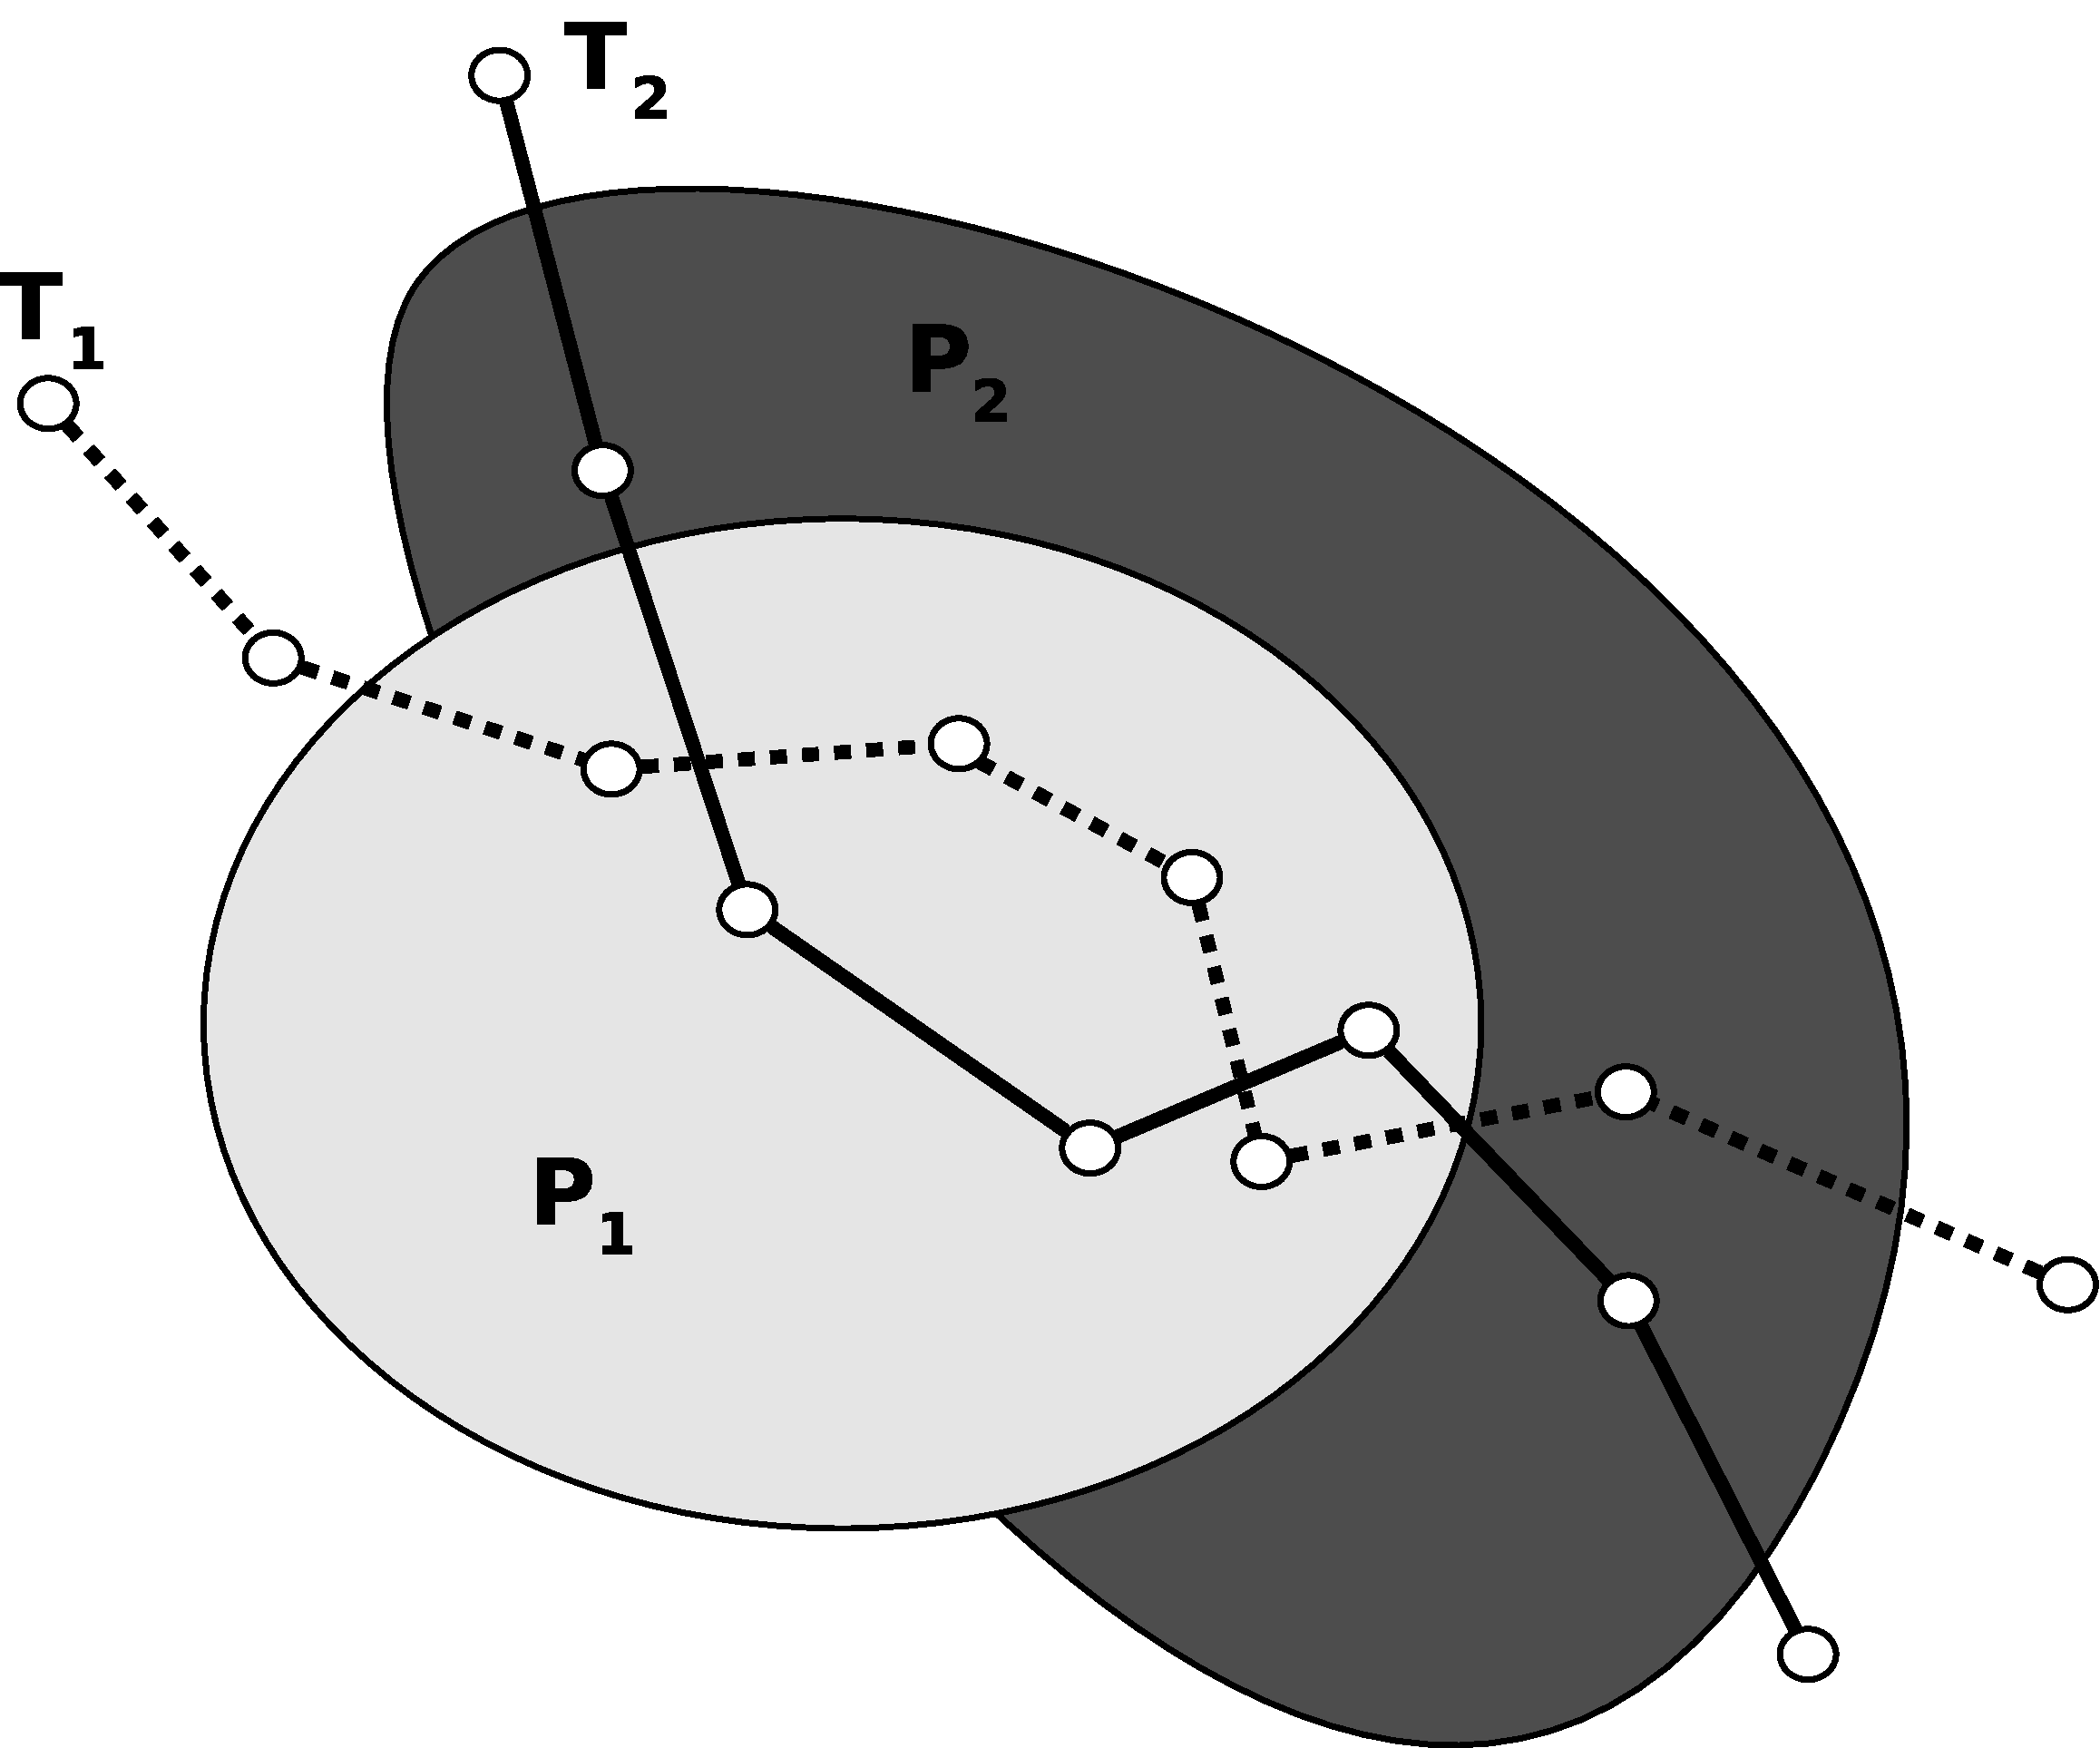
\includegraphics[width=0.3\columnwidth]{figures/poiIntersect.pdf}
      \\
     (a) Aalborg data & (b)  Beijing data
     \end{tabular}
\caption{Hit ratio vs. Levels}
\label{fig:levelVsHitRatio}
\end{figure}